
\documentclass[runningheads,a4paper,11pt]{report}

\usepackage{algorithmic}
\usepackage{algorithm} 
\usepackage{array}
\usepackage{amsmath}
\usepackage{amsfonts}
\usepackage{amssymb}
\usepackage{amsthm}
\usepackage{caption}
\usepackage{comment} 
\usepackage{epsfig} 
\usepackage[T1]{fontenc}
\usepackage{geometry} 
\usepackage{graphicx}
\usepackage[driverfallback=dvipdfm,colorlinks]{hyperref} 
\usepackage[latin1]{inputenc}
\usepackage{multicol}
\usepackage{multirow} 
\usepackage{rotating}
\usepackage{setspace}
\usepackage{subfigure}
\usepackage{url}
\usepackage{verbatim}
\usepackage{indentfirst}
\geometry{a4paper,top=3cm,left=2cm,right=2cm,bottom=3cm}


\newcolumntype{L}[1]{>{\raggedright\let\newline\\\arraybackslash\hspace{0pt}}m{#1}}
\newcolumntype{C}[1]{>{\centering\let\newline\\\arraybackslash\hspace{0pt}}m{#1}}
\newcolumntype{R}[1]{>{\raggedleft\let\newline\\\arraybackslash\hspace{0pt}}m{#1}}


\hypersetup{
pdftitle={artTitle},
pdfauthor={name},
pdfkeywords={pdf, latex, tex, ps2pdf, dvipdfm, pdflatex},
bookmarksnumbered,
pdfstartview={FitH},
urlcolor=cyan,
colorlinks=true,
linkcolor=black,
citecolor=black,
}
\pagestyle{plain}

\setcounter{secnumdepth}{3}
\setcounter{tocdepth}{3}

\linespread{1}

\pagestyle{myheadings}

\makeindex


\begin{document}

\begin{titlepage}
\sloppy
\begin{center}
BABE\c S BOLYAI UNIVERSITY, CLUJ NAPOCA, ROM\^ ANIA

FACULTY OF MATHEMATICS AND COMPUTER SCIENCE

SPECIALIZATION SOFTWARE ENGINEERING 

\vspace{5cm}

\Huge \textbf{Tracking progress of rehabilitation therapy using AI}

\vspace{1cm}

\normalsize -- DISSERTATION THESIS --

\end{center}


\vspace{5cm}

\begin{flushleft}
\textbf{Supervisor} \break
\Large{\textbf{Lect. Dr. Ioan Lazar}}
\end{flushleft}

\begin{flushright}
\textbf{Author} \break
\Large{\textbf{Razvan Timis}}
\end{flushright}

\vspace{4cm}

\begin{center}
2019
\end{center}

\end{titlepage}

\pagenumbering{gobble}

\renewcommand{\contentsname}{Table of Contents}
\tableofcontents

% \newpage

% \listoftables
% \listoffigures
% \listofalgorithms

\newpage

\setstretch{1.5}

\begin{abstract}
\begin{comment}

Scopul acestei lucrări este de a obține rapoarte privind progresul pacienților bazate pe algoritmi inteligenți de estimare a pozitie care să motiveze pacientul să continue recuperarea medicală.

Majoritatea pacienților necesită recuperare medicală pe termen lung, ceea ce înseamnă o medie de 2 sau 3 ani, renunțarea în timpul perioadei de recuperare deoarece nu văd rezultatele chiar dacă acestea există, acestea nu sunt evidente cu ochiul liber.
Mai îngrijorător este faptul că până la 70\% dintre pacienți renunță la fizioterapie, deoarece nu pot vedea rezultate imediate.

Solutia nostra consta in realizarea de doua prototipuri care sa demostreze capacitatea acestor algoritmi de a fi integrati intr-o solutie care sa ajute utilizator final, ne vom axa pe performanta acestor algoritmi.

Principala problema este performanta redusa deoarece necesita un volumn mare de calcule.

Obiectivul este de a rula algoritmi la o performanta de 30 framuri pe secunda pe dispozitivul utilizatorului final.
In continuare am studiat doua arhitecturi importante in pose estimation.

MobileNet care este optimizata pentru mobile, reducand numarul de caulcule.
Convolutional pose machines care este specializata in detectia de posturi, avand o structura composa din mai multe 
clasificatoare.
In acest sens am ales utilizarea in doua aplicati separate a acestor arhitecturi observand performanta si precizia estimarilor.

O aplicatie mobila pentru urmarirea progresului pacientului in timp real folosind camera telefonului. 
Acesta va face fiecare exercitu in fata camerai si va primit raporte legate de performantele lui pe zile.
Performantele insemnand distantele parcurse in timpul exercitiului de membrele copului.


Aplicatie web care va calcula Range of Motion pentru a ajuta pacientul sa faca corect exercitile, astfel vom numara numarul de repatari corecte pe baza unghiurilor care le optine pacientul in timpul exercitiului.
 
In urma implementari celor doua variante am descoperit ca arhitectura retelei prezentate in articolul Convolutional pose machines \cite{DBLP:journals/corr/WeiRKS16} este mai performanta si precisa decat implementarea web folosind  arhitectura MobileNet, care nu este special optimizata pentru problema de pose estimation.
Am obtinut o performata medie de 20 FPS pentru MobileNet in comparatie cu Convolutional pose machines, unde am obtinut 30-60 FPS si o precizie mult mai mare.
 

\end{comment}

\par The goal of this paper is to obtain reports on patient progress based on intelligent pose estimation  algorithms to motivate the patient to continue medical recovery.
\par Most patients require long-term medical recovery, which means an average of 2 or 3 years, give up during the recovery period because they do not see results even if they exist, they are not obvious to the naked eye.
More worrying is that up to 70\% of patients give up physiotherapy because they can not see immediate results.

Our solution consists of making two prototypes demonstrating the ability of these algorithms to integrate into a solution to help the end user, we will focus on the performance of these algorithms.

The main problem is low performance because it requires a large amount of computing.
The objective is to run algorithms at a performance of 30 frames per second on the end-user device.
Next, we studied two important architectures in pose estimation:
\begin{itemize}
    \item MobileNet is optimized for mobile, reducing the number of calculations through special architecture \cite{DBLP:journals/corr/HowardZCKWWAA17}.
    \item Convolutional pose machines that specializes in pose estimation, having a composite structure of several classifiers \cite{DBLP:journals/corr/WeiRKS16}.
\end{itemize}



In this regard, we have chosen to use two separate applications of these architectures, observing the performance and accuracy of the estimates.

The mobile application for tracking patient progress in real time using the camera phone.
He will do each exercise in front of the camera and receive reports related to his performance on days.
The performances are the distances traveled during the exercise by its body members.

The web application will calculate a range of motion to help the patient perform the correct exercises, so we will count the correct number of repetitions of an exercise based on the angles that help the patient during the exercise.

Following the implementation of the two variants, we discovered that the network architecture presented in the article, Convolutional pose machines \cite{DBLP:journals/corr/WeiRKS16}, is more powerful and accurate than the web implementation using the MobileNet architecture, which is not particularly optimized for the pose estimation problem.


This work is the result of my own activity. I have neither given nor
received unauthorized assistance on this work.
\newline\newline
BABEŞ-BOLYAI UNIVERISTY\newline
CLUJ-NAPOCA, JUNE 2019\newline
Timis Razvan Vasile

\end{abstract}

\newpage

\pagenumbering{arabic}

\chapter{Introduction}
\par In Physiotherapy, tracking Range of Motion (ROM) is a standard approach to measuring progress in patient therapy. Often, ROM is measured subjectively and documentation is inconsistent between clinicians. Physios might come to wrong conclusions if ROM is tracked incorrectly between therapy sessions.

\begin{figure}[htbp]
	\centerline{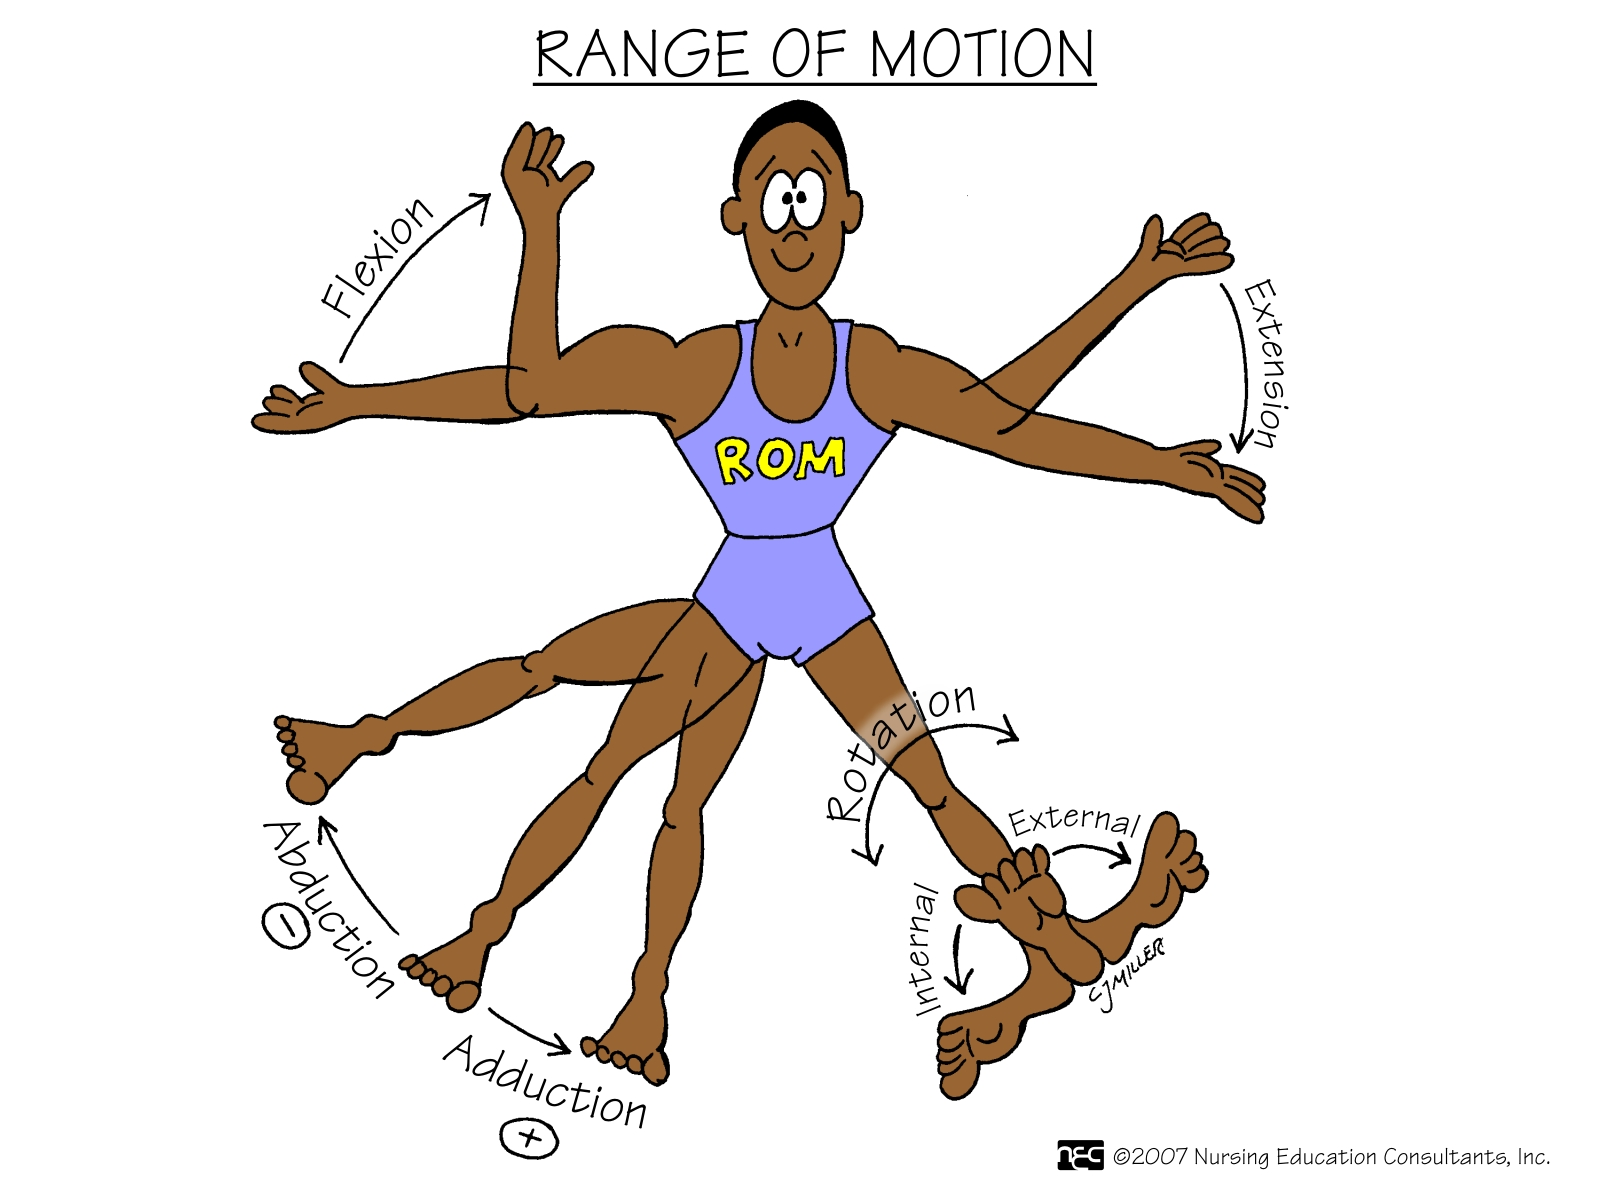
\includegraphics[scale=0.25]{fig/rangeofmotion.png}}  
	\caption{Range of Motion}
\end{figure}

\par The problem is that up to 70\% of patients give up physiotherapy because they can not see immediate results.
\par That's why we want to make a application which makes use of a phone camera to objectively calculate ROM in real-time and automatically produce a report that tracks progress over the course of several therapy sessions.

\section{Motivation}
\par Our motivation is to help patients who need physiotherapy to see a progress and to encourage them to be constant during their treatment. We want to support patients motivation in continuing to build new and healthy behaviours. 
\par This application is designed to help everyone who need physiotherapy treatment to stay motivated, reach their goals, and create habits that are healthy and helpful for a long term. In this case we have a solution by creating a app which will be a useful tool for patients who needs help to reach their goals by automated tracking of ROM.

\section{The purpose of the application}
\chapter{Related work}

\section{DeeperCut\mbox{:} A Deeper, Stronger, and Faster Multi-Person Pose Estimation Model \cite{DBLP:journals/corr/InsafutdinovPAA16}}

\subsection{Problem}
The goal of this paper is to advance the state-of-the-art of articulated pose estimation in scenes with multiple people.

\subsection{Methods}
\par Part Affinity Fields (PAFs), to learn to associate body parts with individuals in the image. The architecture encodes global context, allowing a greedy bottom-up parsing step that maintains high accuracy while achieving realtime performance.	
\par The part affinity is a 2D vector field for each limb: for each pixel in the area belonging to a particular limb, a 2D vector encodes the direction that points from one part of the limb to the other. Each type of limb has a corresponding affinity field joining its two associated body parts.


\subsection{Data}
\par The MPII human multi-person dataset \cite{database2dhuman}  and the COCO 2016 keypoints challenge dataset \cite{coco2016}. These two datasets collect images in diverse scenarios that contain many real-world challenges such as crowding, scale variation, occlusion, and contact.
\par MPII Human Pose dataset is a state of the art benchmark for evaluation of articulated human pose estimation. The dataset includes around 25K images containing over 40K people with annotated body joints. The images were systematically collected using an established taxonomy of everyday human activities.


\subsection{Performance and comparisons}
Evaluation is done on two single-person and two multi-person pose estimation benchmarks. The proposed approach significantly outperforms best known multi-person pose estimation results while demonstrating competitive performance on the task of single person pose estimation.

\section{Human Pose Estimation from Monocular Images: A Comprehensive Survey
\cite{humanmonocular}}

\subsection{Problem}
\par In this paper, a comprehensive survey of human pose estimation from monocular images is carried out including milestone works and recent advancements. The goal of our application is to provide initialization for automatic video surveillance. 
\subsection{Methods}
\par Based on one standard pipeline for the solution of computer vision problems, this survey splits the problem into several modules: feature extraction and description, human body models, and modeling methods. There are additional sections for motion-related methods in all modules: motion features, motion models, and motion-based methods.

\subsection{Data}
The paper collects 26 publicly available datasets for validation and provides error measurement methods that are frequently used.
\subsection{Performance and comparisons}
\par The first survey that includes recent advancements on human pose estimation based on deep learning algorithms. Although deep learning algorithms bring huge success to many computer vision problems, there are no human pose estimation reviews that discuss these works. In this survey, about 20 papers of this category are included. This is not a very large number compared to other problems, but this is a inclusive survey considering the relatively few works addressing this problem.

\section{PersonLab: Person Pose Estimation and Instance Segmentation with a Bottom-Up, Part-Based, Geometric Embedding Model
\cite{DBLP:journals/corr/abs-1803-08225}}

\subsection{Problem}
\par Paper try to solve the task of 2-D pose estimation and instance segmentation of people in multi-person images using an efficient single-shot model based on a box-free bottom-up approach. 
The study contributes to computer vision applications such as smart photo editing, person and activity recognition, virtual or augmented reality, and robotics. 

\subsection{Methods}
 Bottom-up approach for pose estimation and segmentation:
 \begin{itemize}
 \item localizing identity-free semantic entities (individual keypoint proposals or semantic person segmentation labels, respectively)
    \item grouping them into person instances:
    \begin{itemize}
        \item use a greedy decoding process to group them into instances
        \item train network to predict instance-agnostic semantic person segmentation maps
        \item for every person pixel we also predict a set vectors to each of the K keypoints of the corresponding person instance. (corresponding vectors fields can be thought as a geometric embedding representation and induce basins of attraction around each person instance, leading to an efficient association algorithm)
         \begin{itemize}
         \item For each pixel xi, they predict the locations of all K keypoints for the corresponding person that xi belongs to
         \item then compare this to all candidate detected people j (in terms of average keypoint distance), weighted by the keypoint detection probability 
         \item if this distance is low enough, we assign pixel i to person j

         \end{itemize}
    \end{itemize}
 \end{itemize}


\subsection{Data}
Standard COCO keypoint dataset \cite{coco2016} , which annotates multiple people with 12 body and 5 facial keypoints.

\subsection{Performance and comparisons}
\begin{itemize}
    \item compared to the best previous bottom-up approach they improve keypoint AP (Average Precision) from 0.655 to 0.687
    \item compared to the strong top-down FCIS method \cite{DBLP:journals/corr/LiQDJW16} improve mask AP from 0.417 to 0.386
\end{itemize}


\section{Towards Accurate Multi-person Pose Estimation in the Wild
\cite{DBLP:journals/corr/PapandreouZKTTB17}}

\subsection{Problem}
\par Paper try to solve the task of multi-person detection and 2D pose estimation based on a top-down approach (2-D localization of human joints on the arms, legs, and keypoints on torso and the face).
The study want to localize people, understand the activities they are involved in, understand how people move for the purpose of Virtual/Augmented Reality, and learn from them to teach autonomous systems.


\subsection{Methods}
 Top-down approach consisting of two stages:
 \begin{itemize}
    \item first stage, predict the location and scale of boxes which are likely to contain people, use Faster RCNN detector.
    \item second stage, estimate the keypoints of the person potentially contained in each proposed bounding box:
        \begin{itemize}
            \item for each keypoint type predict dense heatmaps and offsets using a fully convolutional ResNet
            \item combine these outputs by a novel aggregation procedure to obtain highly localized keypoint predictions

             \begin{itemize}
             \item use keypoint-based Non-Maximum-Suppression (NMS), instead of the cruder boxlevel NMS
             \item keypoint-based confidence score estimation, instead of box-level scoring
    
             \end{itemize}
        \end{itemize}
 \end{itemize}


\subsection{Data}

Training data: standard COCO keypoint dataset \cite{coco2016}, which annotates multiple people with 12 body and 5 facial keypoints.


\subsection{Performance and comparisons}
\begin{itemize}
    \item average precision of 0.649 on the COCO test-dev set and the 0.643 test-standard sets, outperforming the winner of the 2016 COCO keypoints challenge and other recent state-of-art
    \item using additional in-house labeled data we obtain an even higher average precision of 0.685 on the test-dev set and 0.673 on the test-standard set, more than 5\% absolute improvement compared to the previous best performing method on the same dataset

\end{itemize}



\section{Realtime Multi-Person 2D Pose Estimation using Part Affinity Fields
\cite{DBLP:journals/corr/CaoSWS16}}

\subsection{Problem}
\par The purpose is to recognize a layout of the body parts, based on the pose estimation and Pose Affinity Fields (PAF)



\subsection{Methods}
 \begin{itemize}
    \item Part affinity fields(PAF): is a set of 2D vector fields that encode the location and orientation of the limbs. It is a set of vectors that encodes the direction from one part of the limb to the other; each limb is considered as an affinity field between body parts.
    \item Estimation of body-part confidence maps.
 \end{itemize}
\begin{figure}[htbp]
	\centerline{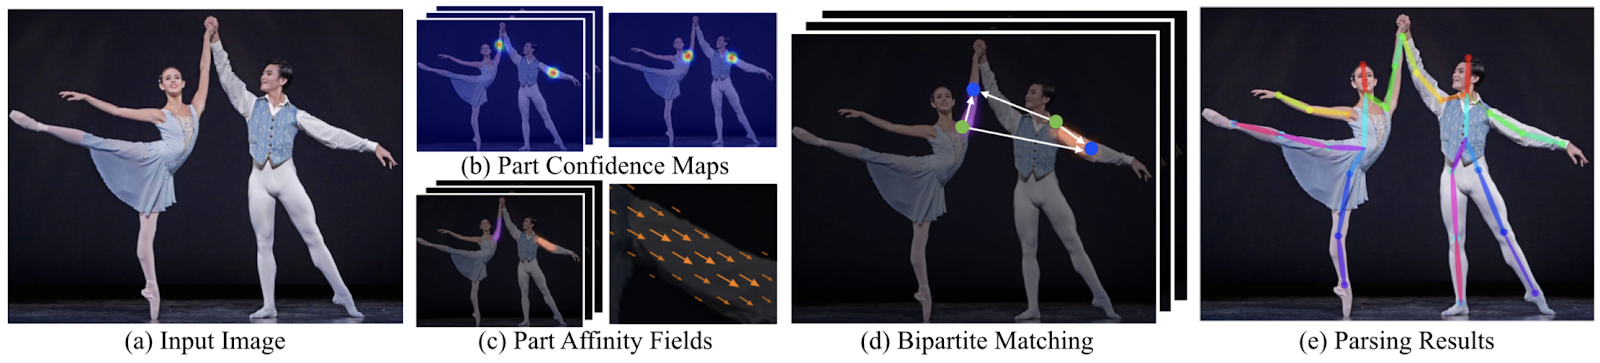
\includegraphics[scale=0.25]{fig/algoritm-ann.png}}  
	\caption{Overall pipeline}
\end{figure}

\subsection{Data}
\par As an input we have an image. This method simultaneously infers two maps with body-parts, as you can see in b figure and runs a special bipartite matching algorithm. In the end it assemble the body parts into full body poses.
\par Training data: standard COCO keypoint dataset \cite{coco2016} and the MPII human multi-person
dataset \cite{database2dhuman}


\chapter{Application}

\par My Kineto application is an interactive software destined for patients who need physiotherapy treatments. Our application guide patient to see how they need to make their exercises in a correct manner. Also, the application count the number of movements. It is based on exercices, because we think that a constant and correct number of movements could be more efficient for patients then just to present them what exercices they need to do. In this manner the application guides each patient during the all period they need to follow their treatment. 
\begin{figure}[htbp]
	\centerline{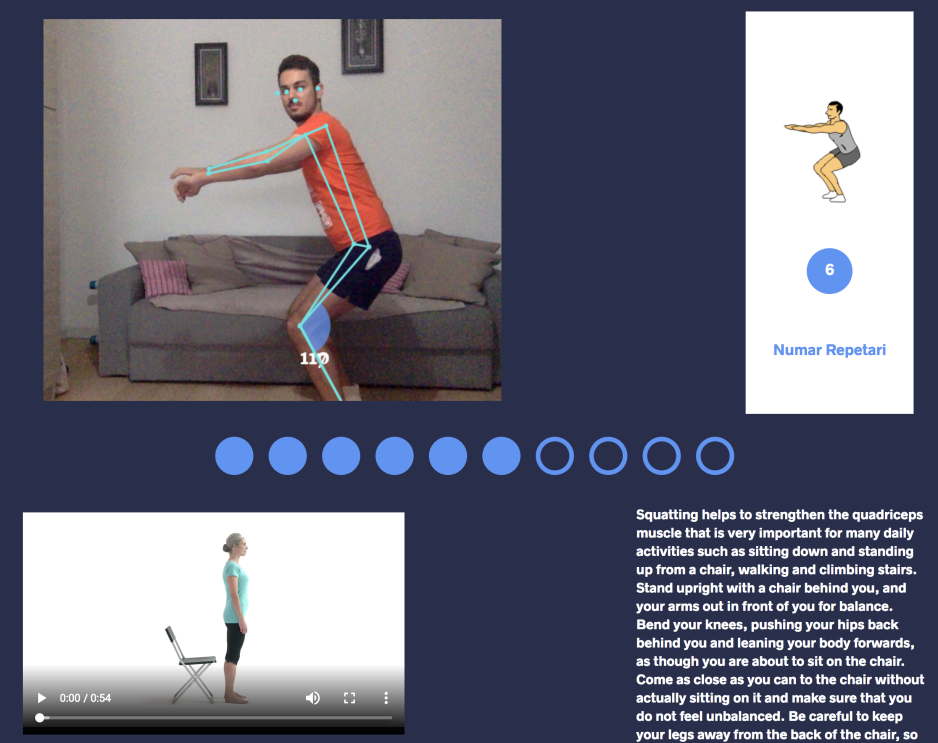
\includegraphics[scale=0.8]{fig/demo-mykineto.png}}  
	\caption{Demo of MyKineto}
\end{figure}
\section{Posture tracking algorithm}

\subsection{Initialization}
Initialization is the first part of the pose tracking algorithm, where we detect the posture with posenet and for each part of the detected skelet we calculate a bounding box and detect the initial set of keypoints that we are going to track in the next steps.
\subsection{Processing}
Processing is composed from three main parts: 
\begin{itemize}
    \item Tracking 
    \item Add new points 
    \item Respawn / Reinitialization
\end{itemize}
This part is used to track as much as possible points detected in the first phase.

\subsection{Keypoints tracking}
\par Points detected in the first part will be used inside tracking algorithm Lucas-Kanade \cite{Lucas:1981:IIR:1623264.1623280} (function calcOpticalFlowPyrLK() from OpenCV). This algorithm fits into the Detect Track  class (DT) and makes a local search to determine the new position of the points of interest detected in the previous frame. For this algorithm to work fine, it's important to take consecutive frames that are easily modified. If we do a sudden move, this algorithm will fail to detect to detect the new position of a part or even all the points in the previous frame. For this case, the next two steps in the algorithm will try to restore the system. 
\par The points in the system that are tracked are detected with Shi-Tomasi "Good features to track" \cite{323798}. 
\par After we detect new position for our keypoints we have to detect the new bounding box that correspond to their new position. For this task we choose to detect the homography matrix based on old points and new points position. Based on homography matrix we calculate the perspective transformation of previous bounding box.
\subsection{Add new points}
\par Adding new points is a step for restoring the system. As we track certain points, we may lose track of some of them. In this case, to prevent destabilization of the system, we will add new key points.
\par The system starts with a maximum number of key points. If a percentage of N of the maximum number of points is lost, then we will try to find others to replace the missing ones. 
\par The detection of new points will be achieved with the Shi-Tomasi algorithm "Good features to track". To narrow the search space of these algorithms, their implementations in OpenCV allow the definition of a mask. \par A mask is an image size matrix in which we want to find the key points. To mark the fact that we want to search in a certain area we will set the value of 1, the mask, in that region and 0 in the rest. Applying a mask is important not only to narrow the search space but also to don\mbox{'}t keep the points detected in an area where our posture skeleton is not found. 
\par More specifically in our application, for each bounding box built from the skelet we will add new points inside it. The calculated bounding box is used to create a mask that we can use inside the keypoints detection algorithm.
\subsection{Respawn / Reinitialization}
\par System reinitialization consists in the identification of the fact that we lost almost all of the tracked points and we are no longer able to estimate, with the remaining number of points, the skeleton posture. The algorithms used to reinitialize the posture are the ones used in the first phase. So basically from this phase if we are no longer able to track and estimate new posture of our skeleton then we go the the first step (Initialization).

\par System reinitialization denotes that the system has been completely destabilized. Loss of a large number of points can occur either due to a sudden movement or because the tracking posture is no longer in the frame.

\begin{figure}
	\centerline{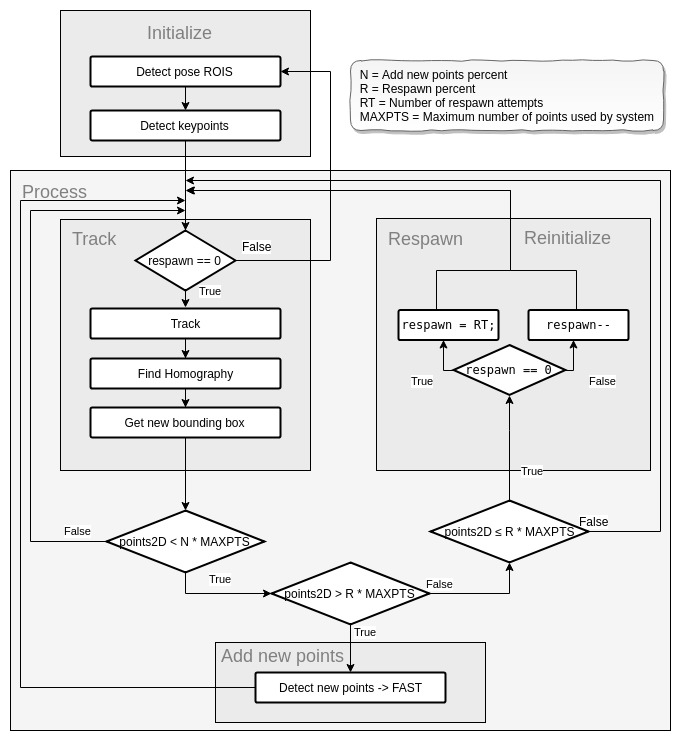
\includegraphics[scale=0.5]{fig/posture-tracking-algorithm.jpg}}  
	\caption{Posture tracking algorithm}
\end{figure}


\chapter{Conclusion}
\par Proposed system for the tracking of the posture doesn\mbox{'}t perform as we originally expected.
\par There seems to be some problems regarding the determination of the bounding box, maybe due to the fact that the detected points are on a surface that is characterized by just a few colors that appear in almost all tracked region. Because of these characteristics of the tracked posture we fail to track enough points due to insufficient difference in the nearest proximity of a point. 

\par For future development we will try to adapt described system to track the contours.

\par Even if posture tracking system doesn\mbox{'}t perform as we expected, we succeeded in the finding the appropriate settings for the PoseNet so that it performs enough good for the determination of the ranges of motion. Based on these calculations we were able to count, in real time, the number of exercises that user made. 


\bibliographystyle{plain}
\bibliography{BibAll}
\end{document}
